\paragraph{QuizziPedia::Front-End::Directives::QuestionTextDirective}

\label{QuizziPedia::Front-End::Directives::QuestionTextDirective}

\begin{figure}[ht]
	\centering
	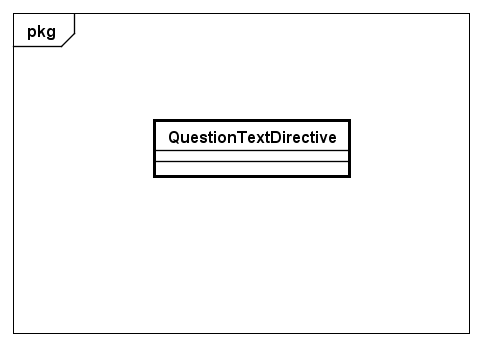
\includegraphics[scale=0.80,keepaspectratio]{UML/Classi/Front-End/QuizziPedia_Front-end_Directives_QuestionTextDirective.png}
	\caption{QuizziPedia::Front-End::Directives::QuestionTextDirective}
\end{figure} 
\FloatBarrier

\begin{itemize}
	\item \textbf{Descrizione}: rappresenta il componente grafico che permette all'utente di scrivere o modificare il testo di una domanda;
	\item \textbf{Utilizzo}: viene usato per permettere all'utente di scrivere o modificare il testo di una domanda;
	\item \textbf{Relazioni con altre classi}: 
	\begin{itemize}
		\item \textit{OUT} \texttt{TrueFalseQuestionsView}: view contenente i campi per creare una domanda vero/falso; 
		\item \textit{OUT} \texttt{MultipleQuestionsView}: view contenente i campi per creare una domanda a risposta multipla;
		\item \textit{OUT} \texttt{ConnectionQuestionsView}: view contenente i campi per creare una domanda a collegamento;
		\item \textit{OUT} \texttt{ImagesSortingQuestionsView}: view contenente i campi per creare una domanda a ordinamento immagini;
		\item \textit{OUT} \texttt{StringsSortingQuestionsView}: view contenente i campi per creare una domanda a ordinamento stringhe;
		\item \textit{OUT} \texttt{FillingQuestionsView}: view contenente i campi per creare una domanda a riempimento testo;
		\item \textit{OUT} \texttt{ClickableAreaQuestionsView}: view contenente i campi per creare una domanda ad area cliccabile;
	\end{itemize}
	\item \textbf{Attributi}: 
	\begin{itemize}
		\item {+ questionText: String} \\ Attributo contenente il testo della domanda;
	\end{itemize}
\end{itemize}